\documentclass[11pt,compress,t,notes=noshow, xcolor=table]{beamer}
\input{../../style/preamble_new}
\input{../../latex-math/basic-math.tex}
\input{../../latex-math/basic-ml.tex}

\title{Deep Learning for NLP}

\definecolor{texblue}{rgb}{0, 0, 1}
\def\myblue#1{\textcolor{texblue}{#1}}
\long\def\devour#1{}

\begin{document}

\titlemeta{
Large Language Models (LLMs)
}{
Explainability and Interpretability
}{
figure/ioi_fig2.png
}{
\item Distinguish feature attribution, training-data attribution, and mechanistic interpretability
\item Explain how LIME, SHAP, and related methods attribute model outputs to input features
\item Understand how training examples and internal model components can be linked to model behavior
\item Distinguish plausible from faithful explanations and describe how explanation quality can be evaluated
}

\begin{vbframe}{Why Explain Model Behavior?}

Interpretability is useful for different reasons:

\begin{itemize}
    \item \textbf{debugging:}
    why did the model fail?

    \item \textbf{model improvement:}
    which features, examples, or components drive behavior?

    \item \textbf{scientific understanding:}
    what representations and mechanisms has the model learned?

    \item \textbf{appropriate reliance:}
    when should users trust or distrust the model?

    \item \textbf{data analysis:}
    which training examples influenced a prediction?
\end{itemize}

\begin{center}
\textbf{Different goals require different kinds of explanations.}
\end{center}

\citebutton{Calderon \& Reichart, 2025}
{https://aclanthology.org/2025.naacl-long.29/}

\end{vbframe}


\begin{vbframe}{Different Stakeholders and Goals}

Interpretability is useful for different stakeholders and purposes.

\begin{figure}
    \centering
    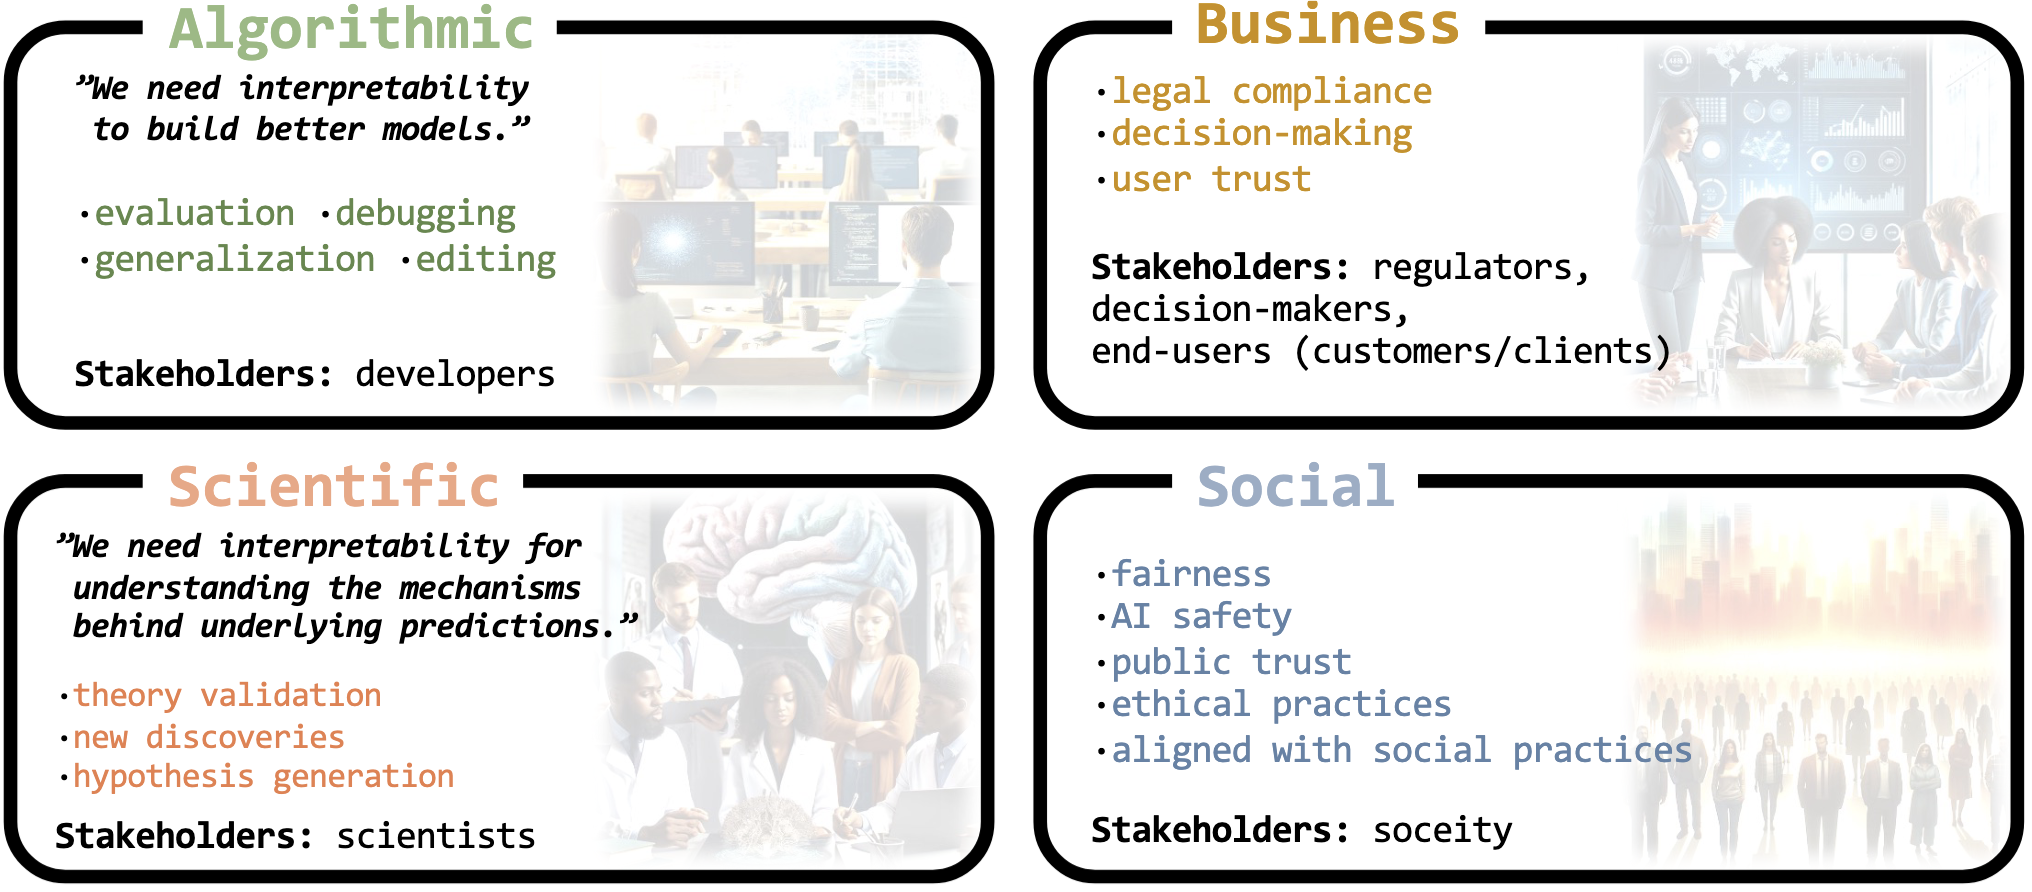
\includegraphics[width=10.8cm]
    {figure/interpretability_stakeholders_fig2.png}
\end{figure}

\citebutton{Calderon \& Reichart, 2025}
{https://aclanthology.org/2025.naacl-long.29/}

\end{vbframe}


\begin{vbframe}{What Kind of Explanation?}

The same model behavior can be explained in different ways.

\begin{description}

    \item[\textbf{Feature attribution}]
    Which parts of the input influenced the output?
    \[
    x_j \longrightarrow f(x)
    \]

    \item[\textbf{Training-data attribution}]
    Which training examples influenced the output?
    \[
    z_i^{\mathrm{train}}
    \longrightarrow
    \theta
    \longrightarrow
    f_\theta(x)
    \]

    \item[\textbf{Mechanistic interpretation}]
    Which internal components and causal pathways produce the behavior?
    \[
    \text{activations / heads / features}
    \longrightarrow
    f_\theta(x)
    \]

\end{description}

Explanations may additionally be\\

\textbf{local} (specific to a single input)\\
or\\
\textbf{global} (independent of a specific input).

\end{vbframe}

% ------------------------------------------------------------------------------
\begin{frame}[plain]
\vfill
\begin{center}
{\LARGE \textbf{Feature Attribution}}
\end{center}
\vfill
\end{frame}
% ------------------------------------------------------------------------------

\begin{vbframe}{Feature Attribution: What Does It Look Like?}

Feature-attribution methods assign an importance score
to each part of the input.

\begin{figure}
    \centering
    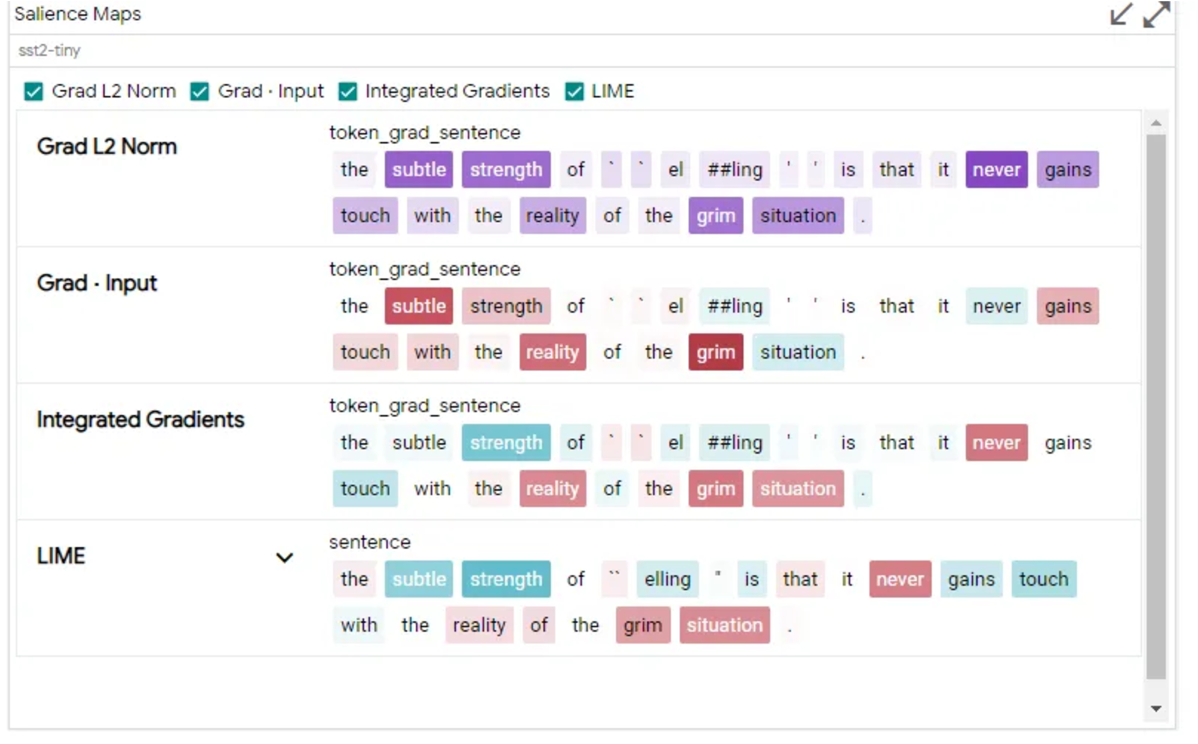
\includegraphics[width=0.6\textwidth]
    {figure/feature_attribution_example.png}
\end{figure}

Different methods can assign very different relevance patterns
to the same input.

\end{vbframe}

% ------------------------------------------------------------------------------

\begin{vbframe}{Gradient-Based Attribution}

Let \(S(x)\) be a scalar model output, such as
the logit of a target class.

For token representation \(e_j\),

\[
\nabla_{e_j} S(x)
\]

measures how sensitive the output is to a small change
in that token representation.

Using a first-order Taylor approximation,

\[
S(x+\Delta x)
\approx
S(x)
+
\nabla_x S(x)^\top \Delta x.
\]

\begin{center}
\textbf{Large gradient}
\(\Rightarrow\)
\textbf{large local sensitivity.}
\end{center}

\end{vbframe}


% ------------------------------------------------------------------------------
% #3c
% ------------------------------------------------------------------------------

\begin{vbframe}{Gradient Attribution: Advantages and Limitations}

\textbf{Advantages}

\begin{itemize}
    \item one backward pass,
    \item supported directly by automatic differentiation,
    \item no perturbation sampling,
    \item no auxiliary explanation model.
\end{itemize}

\medskip

\textbf{Limitation}

Gradients describe \emph{infinitesimal} changes in embedding space.

\[
e_j
\longrightarrow
e_j+\epsilon
\]

But natural-language features are discrete:

\[
\text{word present}
\quad\text{or}\quad
\text{word removed}.
\]

\begin{center}
\textbf{This motivates perturbation-based explanations.}
\end{center}

\end{vbframe}


% ------------------------------------------------------------------------------

\begin{vbframe}{LIME: Local Perturbations}

Consider

\[
x=
\text{``This was not a movie I did enjoy.''}
\]

Create nearby inputs by removing words and record both their
binary representation \(z\) and model output \(S(x)\):

\[
\begin{array}{lll}
\textbf{perturbed input} & \textbf{encoding } z & \textbf{model output } S(x)\\
\hline
\text{This was not a movie I did enjoy}
&
[1\,1\,1\,1\,1\,1\,1\,1]
&
0.88
\\[0.3em]

\text{This was a movie I did enjoy}
&
[1\,1\,0\,1\,1\,1\,1\,1]
&
0.21
\\[0.3em]

\text{This was enjoy}
&
[1\,1\,0\,0\,0\,0\,0\,1]
&
0.15
\\[0.3em]

\text{not a movie I enjoy}
&
[0\,0\,1\,1\,1\,1\,0\,1]
&
0.73
\end{array}
\]

Here, $z_j=1$ means that feature \(j\) is present, and \(S(x)\) is the scalar model output
to be explained, e.g. the probability of the negative class.

%\begin{center}
%\textbf{LIME learns from these perturbed input--output pairs.}
%\end{center}

%\citebutton{Ribeiro et al., 2016: LIME}
%{https://arxiv.org/abs/1602.04938}

\end{vbframe}


% ------------------------------------------------------------------------------

\begin{vbframe}{LIME: Objective Function}

        Local explanation of the model output \(S(x)\): $\hat S(z)=\mathbf w^\top z$


        LIME chooses the explanation weights by

        \[
        \boxed{
        \mathbf w^*
        =
        \argmin_{\mathbf w}
        \sum_{i=1}^{N}
        \pi_i
        \left[
        S(x^{(i)})
        -
        \mathbf w^\top z^{(i)}
        \right]^2
        +
        R(\mathbf w)
        }
        \]

\begin{columns}[T,onlytextwidth]

    \begin{column}{0.48\textwidth}

        where

        \begin{itemize}
            \item \(\pi_i\): weight of perturbation \(i\),
            e.g. larger for inputs closer to the original input,

            \item \(R(\mathbf w)\): regularizer favoring a simple explanation,

            \item \(w_j\): attribution assigned to feature \(j\).
        \end{itemize}

    \end{column}

    \begin{column}{0.48\textwidth}
            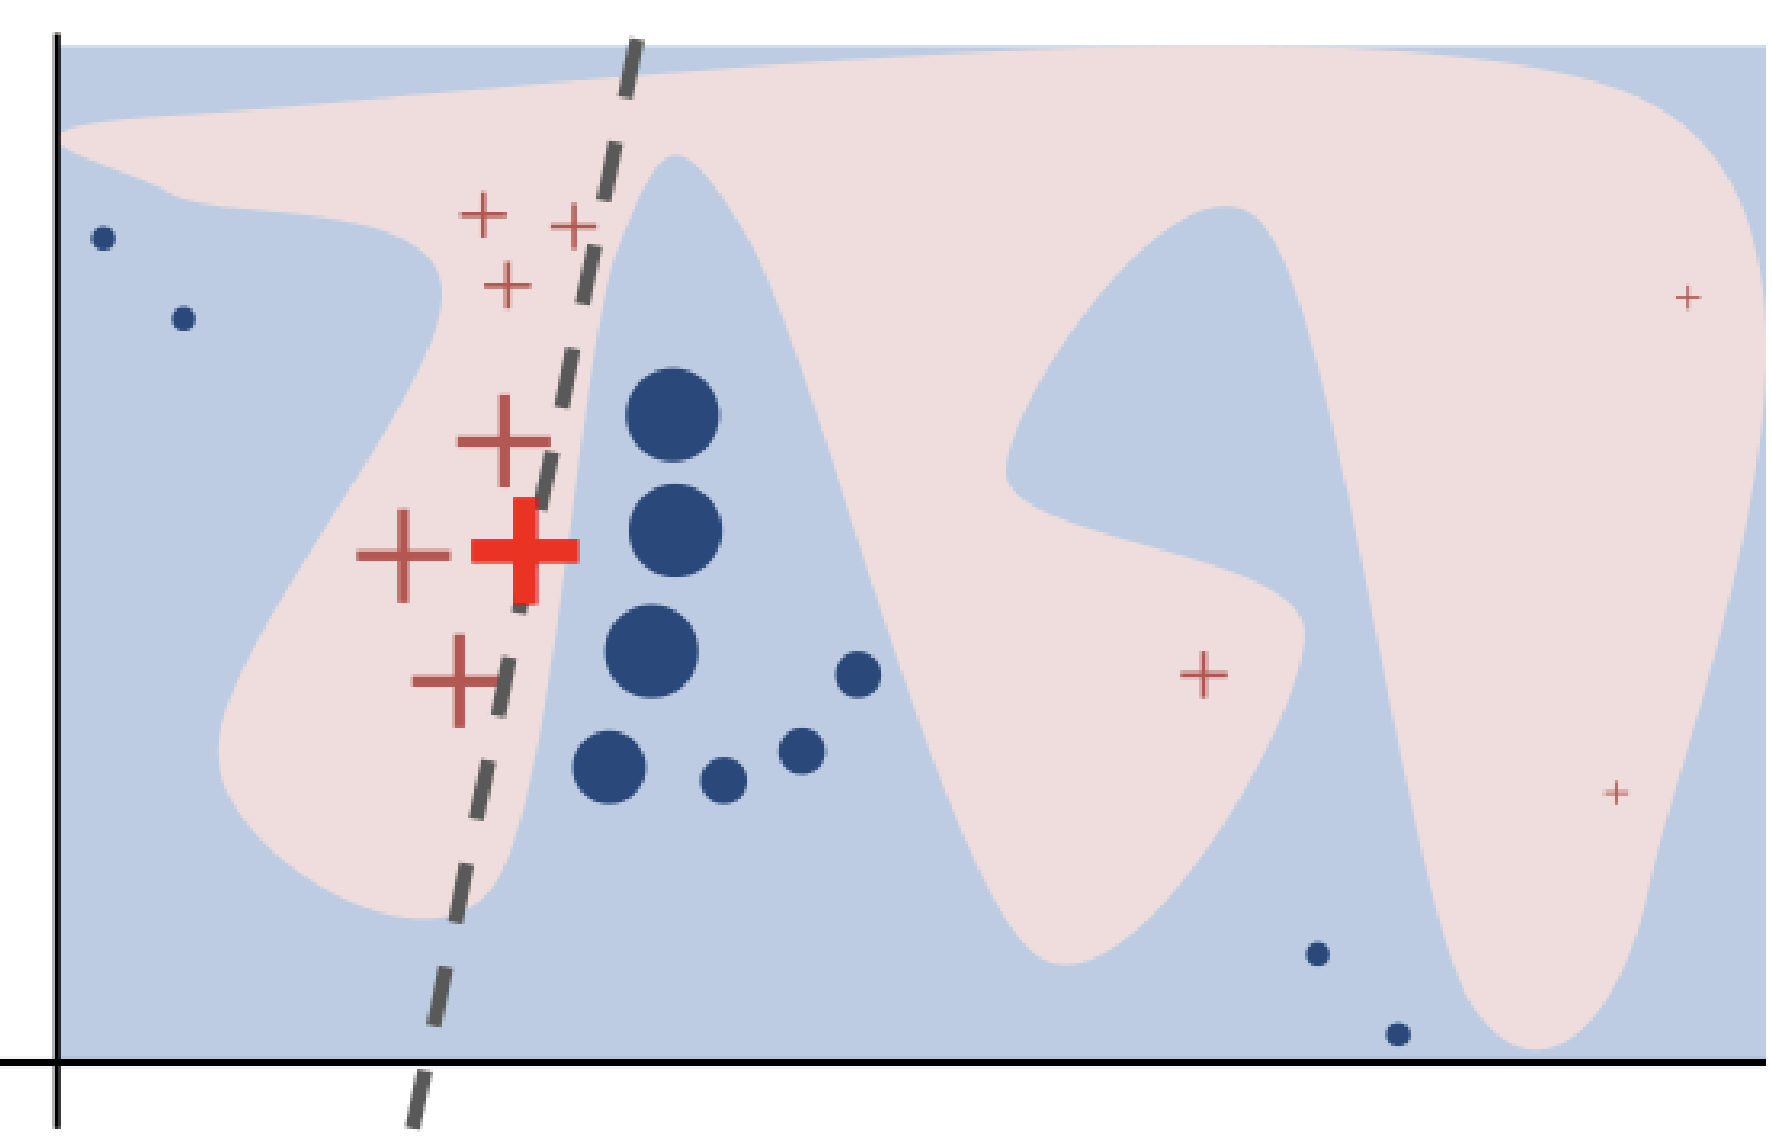
\includegraphics[width=\linewidth]
            {figure/lime_local_approximation_fig3.png}

        %\begin{center}
        %\small
        %Complex model locally approximated
        %by a simple explanation model.
        %\end{center}

    \end{column}

\end{columns}

\end{vbframe}


% ------------------------------------------------------------------------------
% #5b
% ------------------------------------------------------------------------------

\begin{vbframe}{LIME: Practical Details}

For fixed perturbations and weights,

\[
\mathbf w^*
\]

can be obtained with weighted least squares.

The practical difficulty is obtaining enough model evaluations

\[
S(x^{(1)}),\ldots,S(x^{(N)}).
\]

In practice, LIME may require \textbf{thousands of perturbations}
for one explanation.

\medskip

Important design choices remain:

\begin{itemize}
    \item How should the locality weights \(\pi_i\) be chosen?
    \item How strongly should \(R(\mathbf w)\) favor simplicity?
\end{itemize}

\begin{center}
\textbf{SHAP fixes these choices in a principled way.}
\end{center}

\end{vbframe}

% ------------------------------------------------------------------------------

\begin{vbframe}{SHAP: The Game-Theoretic Idea}

\begin{columns}[T,onlytextwidth]

    \begin{column}{0.52\textwidth}

        Think of input features as players in a cooperative game.
    \end{column}

    \begin{column}{0.44\textwidth}

        \begin{figure}
        \centering
        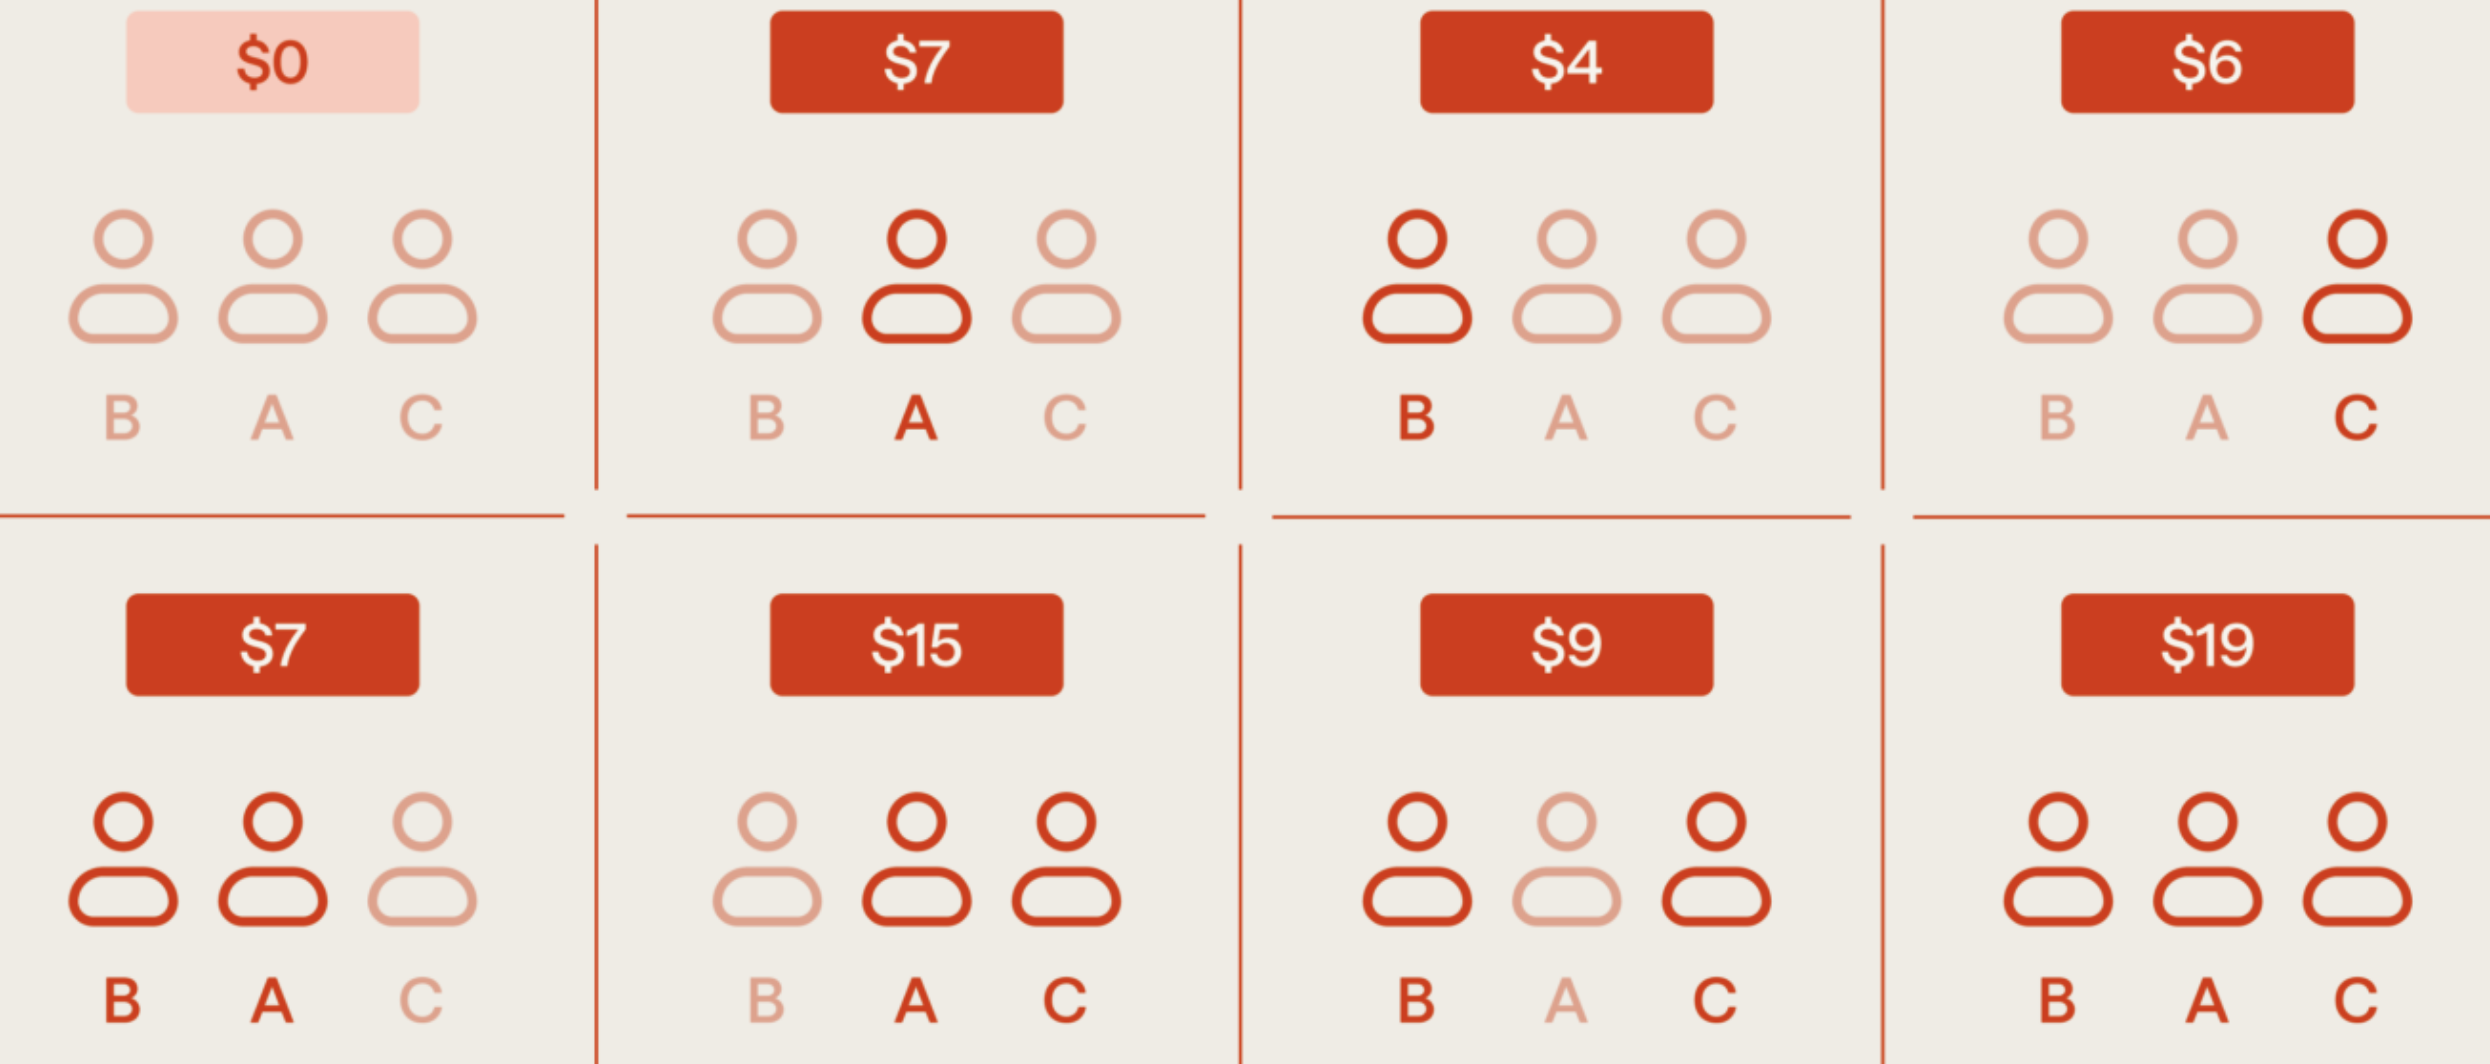
\includegraphics[width=\linewidth]
        {figure/shap_game_theory.png}
        \end{figure}

    \end{column}

\end{columns}

        For player \(s\), ask:
\[
        \text{How much value does } s
        \text{ add in different coalitions with other players?}
        \]

        For a coalition \(A\),

        \[
        S(A\cup\{s\})-S(A)
        \]

        is the marginal contribution of \(s\).
\end{vbframe}


% ------------------------------------------------------------------------------

\begin{vbframe}{SHAP: The Game-Theoretic Idea}

\begin{columns}[T,onlytextwidth]

    \begin{column}{0.52\textwidth}

        Consider again

        \[
        x^{(0)}
        =
        \text{``This was not a movie I did enjoy.''}
        \]

        Suppose the feature to explain is

        \[
        s=\text{``not''}.
        \]

        SHAP asks how much adding \(s\) changes the scalar model output
        \(S(\cdot)\).

    \end{column}

    \begin{column}{0.44\textwidth}

        \begin{figure}
            \centering
            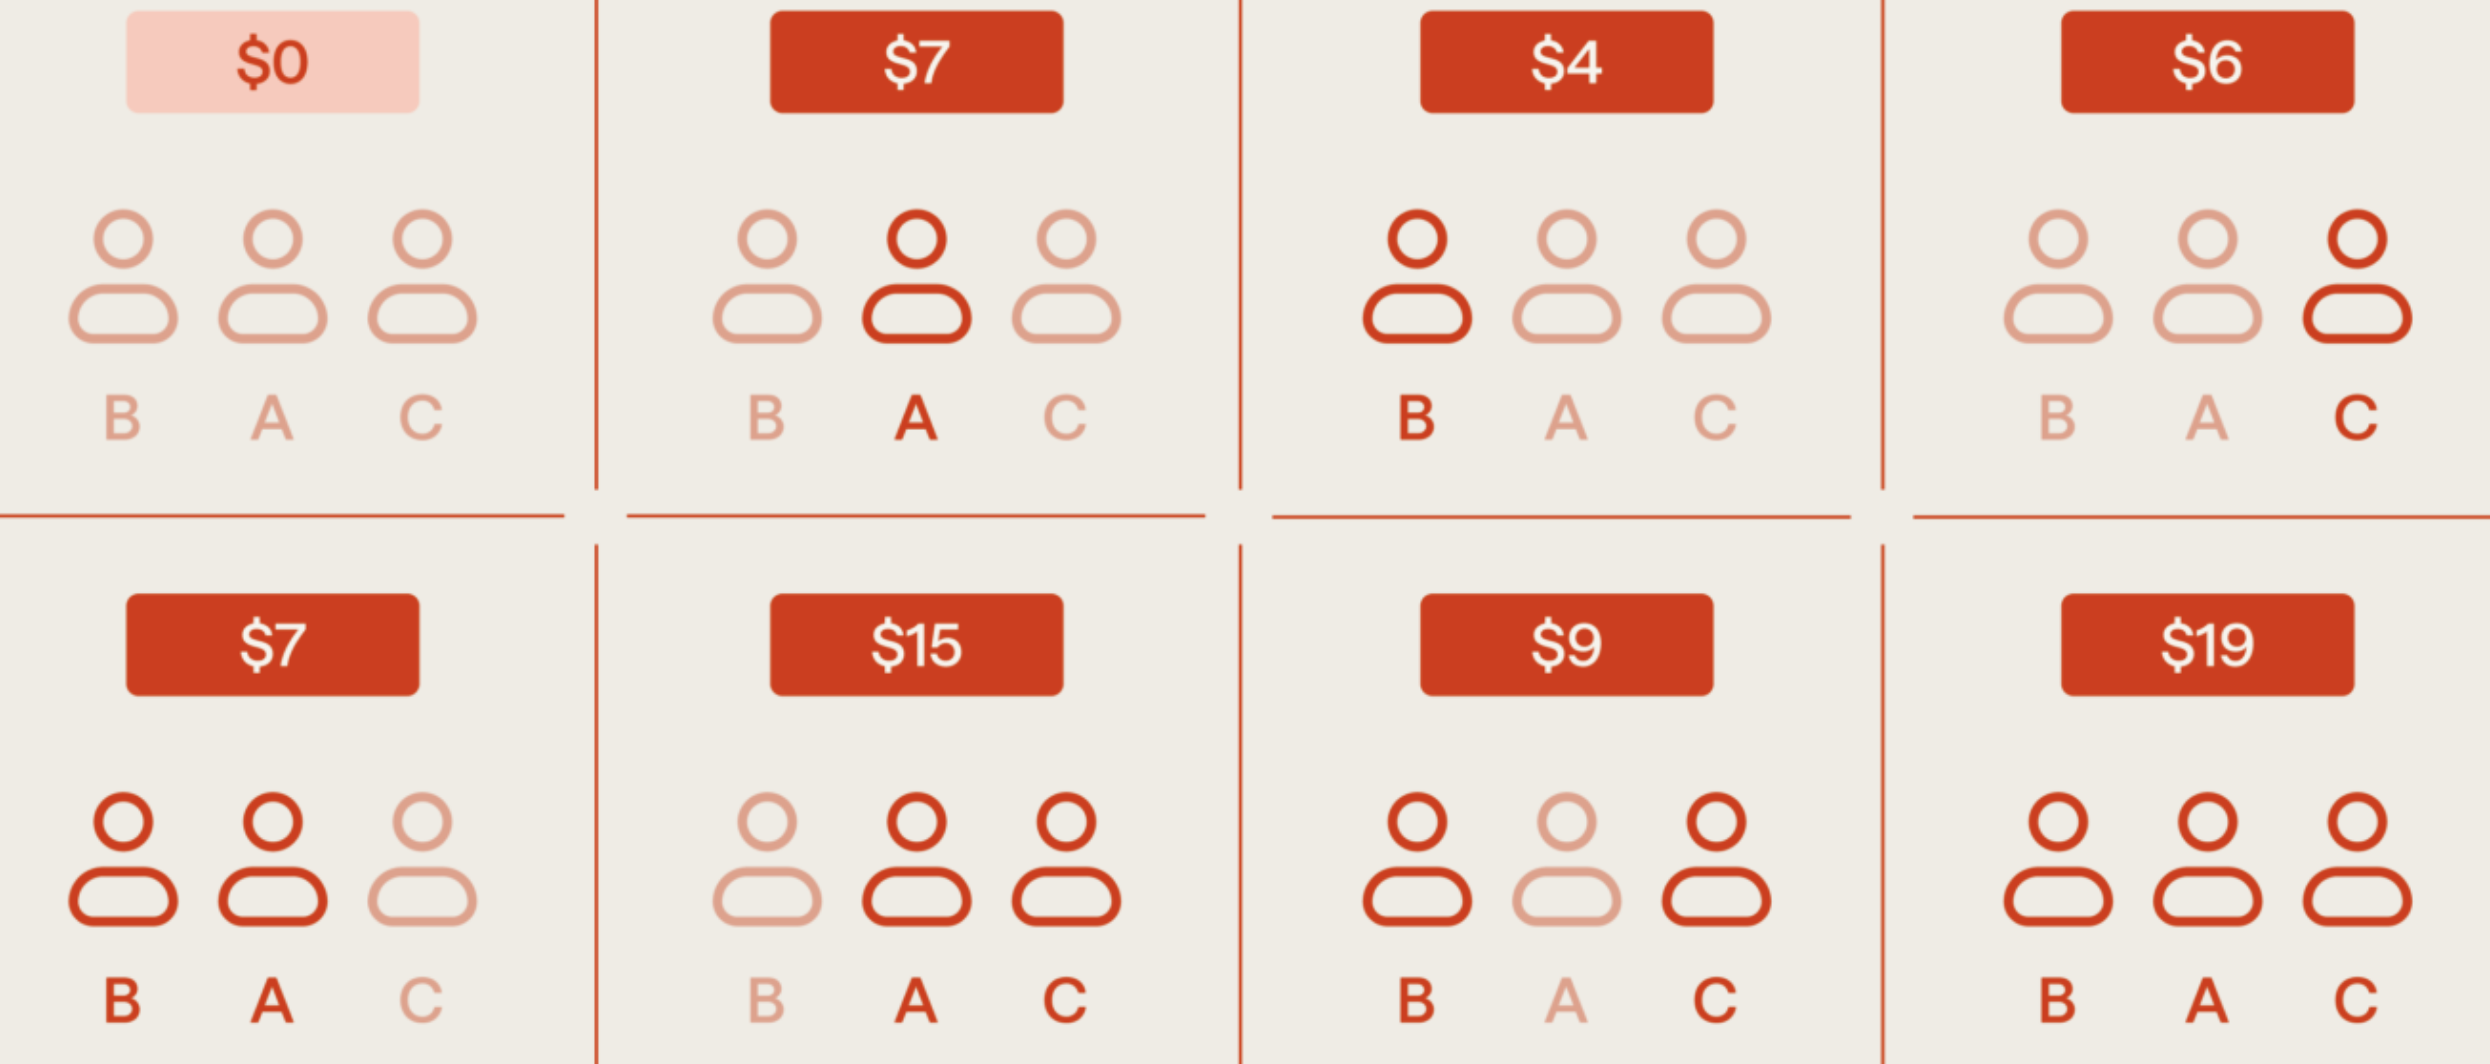
\includegraphics[width=\linewidth]
            {figure/shap_game_theory.png}
        \end{figure}

    \end{column}

\end{columns}

For a subset \(A\) of the other features, compare

\[
\underbrace{S(x(A\cup\{s\}))}_{\text{with ``not''}}
-
\underbrace{S(x(A))}_{\text{without ``not''}}.
\]
\end{vbframe}


% ------------------------------------------------------------------------------

\begin{vbframe}{SHAP: Shapley Attribution}

Let \(M\) be the number of input features.

The SHAP attribution of feature \(s\) is

\[
\boxed{
w_s
=
\sum_{A\subseteq F\setminus\{s\}}
\pi_{\mathrm{SHAP}}(A) 
\left[
S(x(A\cup\{s\}))
-
S(x(A))
\right]
}
\]

where

\begin{itemize}
    \item \(A\): subset of features not containing \(s\),
    \item $\pi_{\mathrm{SHAP}}(A)$: weight for coalition $A$,
    \item \(x(A)\): input containing only features in \(A\),
    \item \(S(x)\): scalar model output,
    \item \(w_s\): attribution assigned to feature \(s\).
\end{itemize}

\end{vbframe}

% ------------------------------------------------------------------------------

\begin{vbframe}{SHAP: Details}

\textbf{Complexity}

Exact SHAP is exponential in the number of features: $2^M$ coalitions for \(M\) features.

In practice, SHAP samples coalitions;
the original paper uses up to \textbf{50,000 samples per explanation}.

\medskip

\textbf{Consistency}

\[
\text{larger marginal contribution}
\;\Rightarrow\;
\text{larger or equal attribution}
\]

\medskip

\textbf{Kernel SHAP - LIME equivalence}

The same Shapley attribution vector is obtained from LIME with $R(\mathbf w)=0$ and $\pi_{\mathrm{Kernel}}(A)
=
\frac{M-1}
{\binom{M}{|A|}\,|A|\,(M-|A|)}.
$

\end{vbframe}

% ------------------------------------------------------------------------------


\begin{vbframe}{Kernel SHAP: Which Perturbations Matter Most?}

Assume an input with \(M=8\) features: $x=
\text{``This was not a movie I did enjoy.''}$

Consider the following perturbations:

\[
\begin{array}{c|c|l}
\textbf{coalition} & \textbf{binary encoding} & \textbf{perturbed input}\\
\hline
A_1 &
[1\,0\,0\,0\,0\,0\,0\,0] &
\text{This}
\\[0.2em]

A_2 &
[1\,1\,1\,1\,0\,0\,0\,0] &
\text{This was not a}
\\[0.2em]

A_3 &
[1\,1\,1\,1\,1\,1\,1\,0] &
\text{This was not a movie I did}
\\[0.2em]

A_4 &
[0\,1\,0\,1\,1\,0\,1\,0] &
\text{was a movie did}
\\[0.2em]

%A_5 &
%[1\,1\,1\,1\,1\,0\,0\,0] &
%\text{This was not a movie}
\end{array}
\]

Kernel SHAP assigns $\pi_{\mathrm{Kernel}}(A)
=
\frac{7}
{\binom{8}{|A|}\,|A|\,(8-|A|)}$

\begin{center}
\ques Rank \(A_1,\ldots,A_5\) from
\textbf{highest} to \textbf{lowest} weight.
\end{center}

\end{vbframe}

\begin{vbframe}{Generative LLMs}

\begin{columns}[T]
\begin{column}{0.5\textwidth}

\vspace{0.2cm}

LIME/SHAP for LLMs:

\begin{itemize}
  \item long input context (e.g., conversations or documents)
  \item generated text output
\end{itemize}

\medskip

So we need:

\begin{itemize}
  \item larger input units\\
        (phrases, sentences, paragraphs)
  \item a scalar output \(S(x)\)
\end{itemize}

\medskip

\citebutton{Paes et al., 2024}{https://arxiv.org/abs/2403.14459}

\end{column}

\begin{column}{0.48\textwidth}
\centering

\includegraphics[width=\linewidth]{figure/long_generation.png}
\end{column}
\end{columns}

\end{vbframe}

% ------------------------------------------------------------------------------

\begin{vbframe}{Scalarizers}

For generated text, we need to map the output to a single score:

\[
S(x) \in \mathbb{R}
\]

\medskip

\textbf{If model probabilities are available:}

\[
S(x)=\log p\!\left(y^{(0)} \mid x\right)
\]

\smallskip

Likelihood of the original generation \(y^{(0)}\).

\bigskip

\textbf{If model probabilities are not available:}

\[
y=f(x),
\qquad
S(x)=\operatorname{sim}\!\left(y,y^{(0)}\right)
\]

\smallskip

Similarity between the new and original generation.

%\bigskip

%\textbf{The explanation depends on what the scalarizer measures.}

\citebutton{Paes et al., 2024}
{https://arxiv.org/abs/2403.14459}

\end{vbframe}


% ------------------------------------------------------------------------------

\begin{vbframe}{MExGen}
MExGen adapts perturbation-based explanations to long-context generation.
\[
\text{large context units}
\;\longrightarrow\;
\text{relevant regions}
\;\longrightarrow\;
\text{finer-grained attribution}
\]
\citebutton{Paes et al., 2024}
{https://arxiv.org/abs/2403.14459}
\begin{columns}
\begin{column}{0.55\textwidth}
\begin{itemize}
  \item start with coarse units such as paragraphs or sentences
  \item identify the most relevant regions
  \item refine only those regions at a finer level
\end{itemize}
\end{column}

\begin{column}{0.45\textwidth}
\begin{center}
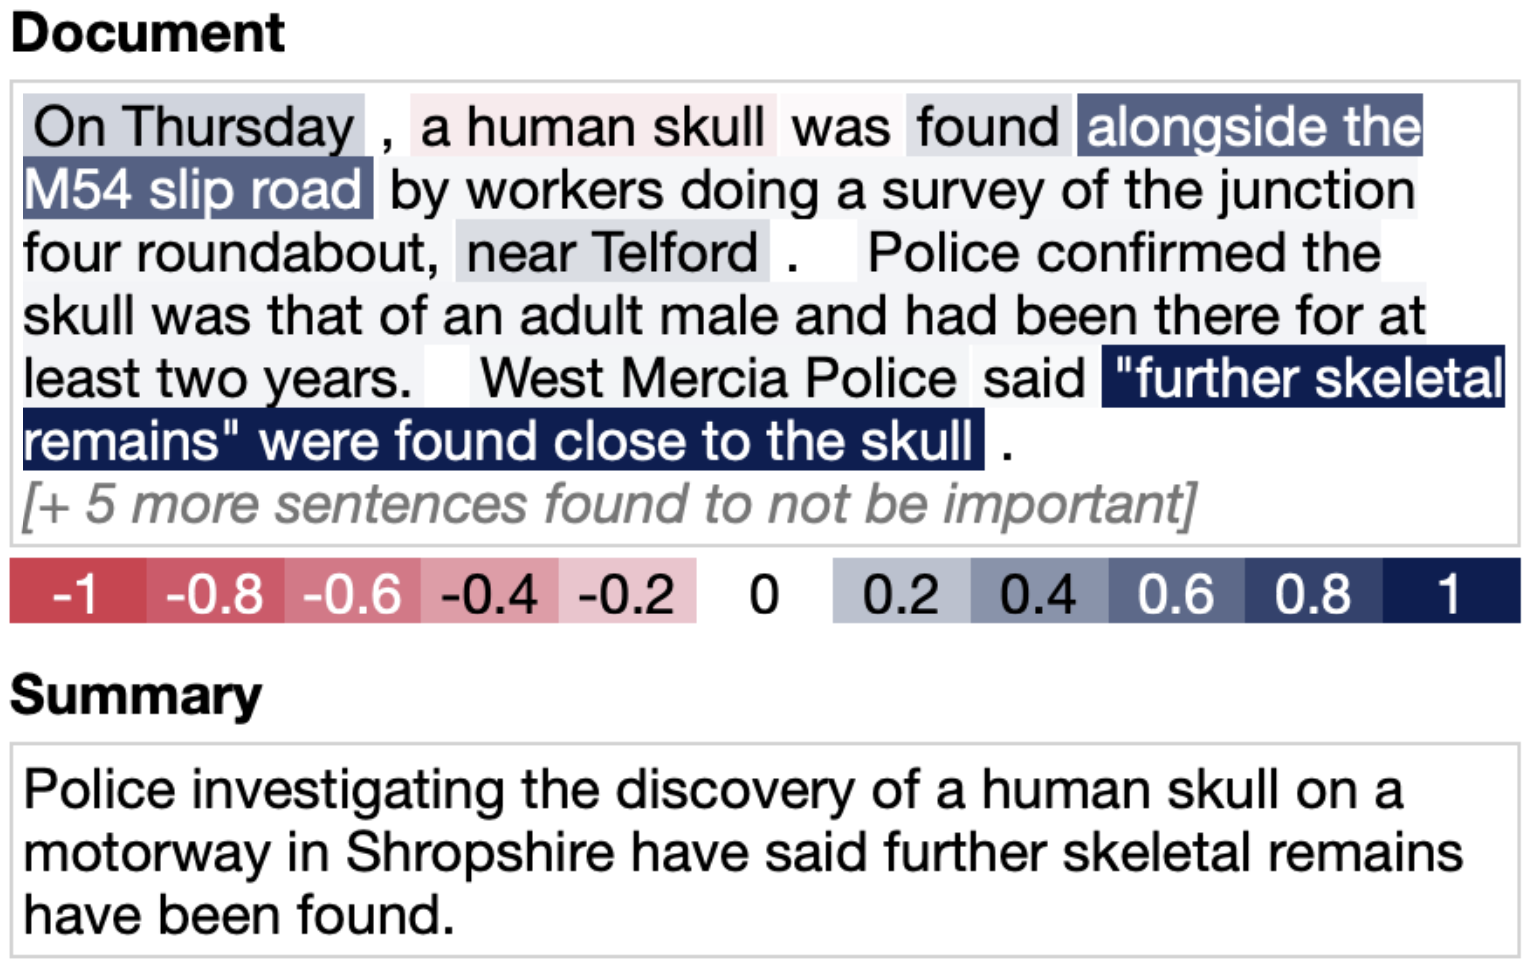
\includegraphics[width=\linewidth]{figure/mexgen_fig1.png}
\end{center}
\end{column}
\end{columns}
This avoids exploring all fine-grained feature subsets and keeps the
number of model queries approximately linear in the number of features.

\end{vbframe}


% ------------------------------------------------------------------------------
\begin{frame}[plain]
\vfill
\begin{center}
{\LARGE \textbf{Training-Data Attribution}}
\end{center}
\vfill
\end{frame}
% ------------------------------------------------------------------------------


% ------------------------------------------------------------------------------ ------------------------------------------------------------------------------

\begin{vbframe}{Training Data Attribution}

\begin{columns}[T]

\begin{column}{0.58\textwidth}

Main question: \textbf{Which training examples influenced this output?}

\medskip

Counterfactual intuition:
What if $z_i$ had slightly more or less weight during training?

\medskip

\citebutton{Grosse et al., 2023}
{https://arxiv.org/abs/2308.03296}

\end{column}

\begin{column}{0.4\textwidth}

\centering
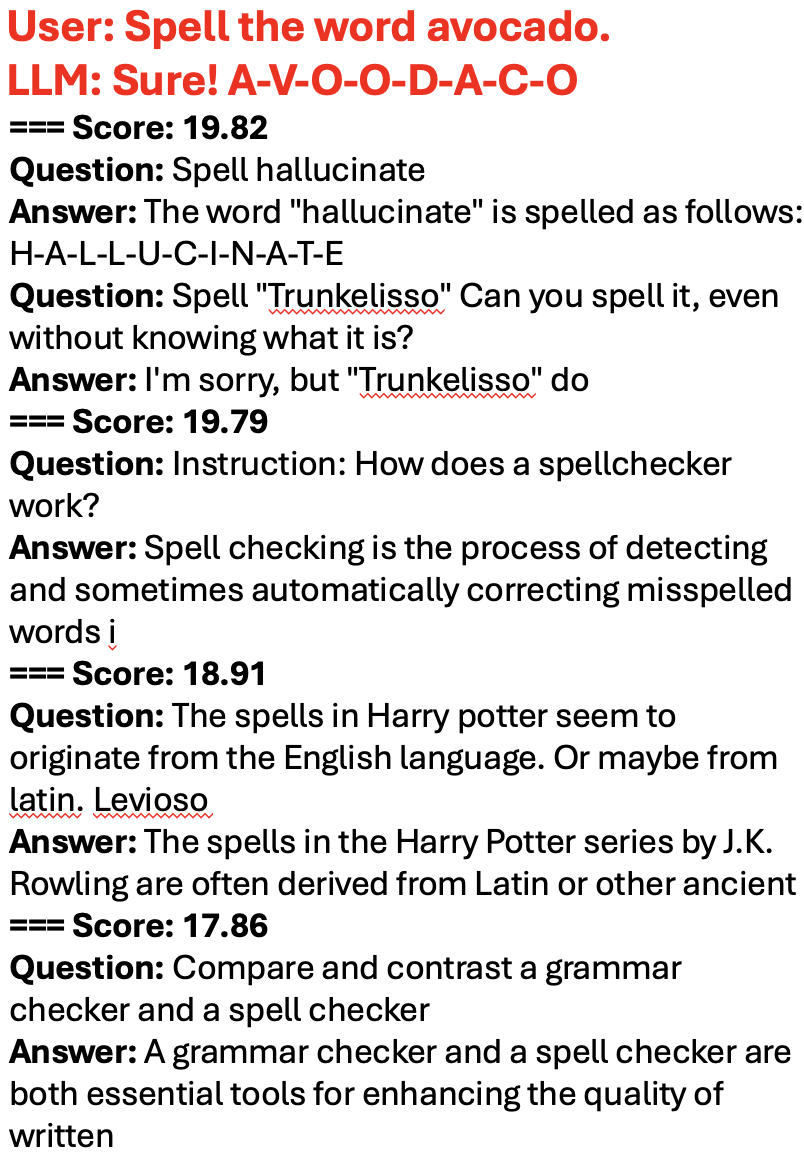
\includegraphics[width=\linewidth]{figure/training_data_attribution_example.png}

\footnotesize{(Actual training examples retrieved from the OLMo-mix dataset,  using Elasticsearch.)}

\end{column}

\end{columns}

\end{vbframe}


% ------------------------------------------------------------------------------

\begin{vbframe}{Influence Functions}

Effect of upweighting training example \(z_i\):

\[
I(z_i,z)
=
-
\nabla_\theta L(z)^\top
H^{-1}
\nabla_\theta L(z_i)
\]

\begin{itemize}
  \item \(\nabla_\theta L(z_i)\): training-example gradient
  \item \(H^{-1}\): inverse Hessian
  \item \(\nabla_\theta L(z)\): gradient of the output to explain
\end{itemize}

\[
\text{Influence}
\approx
\text{effect on target loss when } z_i \text{ gets more weight}
\]

\citebutton{Grosse et al., 2023}
{https://arxiv.org/abs/2308.03296}

A simple approximation drops the inverse Hessian:

\[
I(z_i,z)
\approx
-
\nabla_\theta L(z)^\top
\nabla_\theta L(z_i)
\]
\citebutton{Pruthi et al., 2020}
{https://arxiv.org/abs/2002.08484}

Intuition: $\text{similar gradients}
\;\Longrightarrow\;
\text{high effect on the model}$

\end{vbframe}


% ------------------------------------------------------------------------------

\begin{vbframe}{Why Is This Still Expensive?}

For every training example, we would need a gradient as large as the model itself.

\begin{itemize}
  \item Llama 3 70B: one gradient is roughly 140 GB
  \item OLMo-mix: about 3 billion training documents
  \item computing all training gradients takes roughly as long as training
\end{itemize}

Storing one gradient per training example would require approximately

\[
3 \cdot 10^9 \times 140\text{ GB}
=
4.2 \cdot 10^{11}\text{ GB}.
\]

\end{vbframe}

% ------------------------------------------------------------------------------

\begin{vbframe}{Making Attribution Practical}
Training-data attribution can be approximated: \citebutton{Lin et al., 2024}
{https://arxiv.org/abs/2405.11724}

\begin{columns}

\begin{column}{0.53\textwidth}

\begin{itemize}
  \item \textbf{Two-stage retrieval:} first retrieve similar training examples, then compute influence only for the top candidates
  \item \textbf{Restrict the training set:} consider only a relevant subset, e.g.\ instruction-tuning data
  \item \textbf{Compress gradients:} store lower-dimensional projections instead of full gradients
\end{itemize}
\end{column}

\begin{column}{0.45\textwidth}

\centering
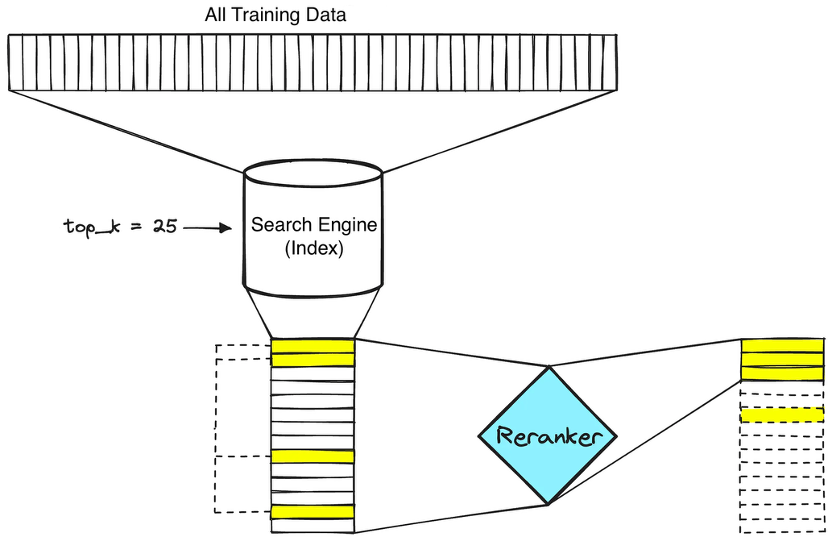
\includegraphics[width=\linewidth]{figure/two_stage_retrieval.png}

\end{column}

\end{columns}

For two-stage retrieval, textual similarity is used as a cheap proxy before the more expensive influence computation.

\end{vbframe}


\begin{vbframe}{Influence at LLM Scale}
Grosse et al. scale influence functions to models with up to 52B parameters.
\begin{columns}
\begin{column}{0.35\textwidth}
\begin{itemize}
  \item TF-IDF prefiltering reduces the candidate set
  \item influential training examples can be highly concentrated
  \item larger models show more abstract forms of influence
\end{itemize}
\end{column}

\begin{column}{0.65\textwidth}

\centering
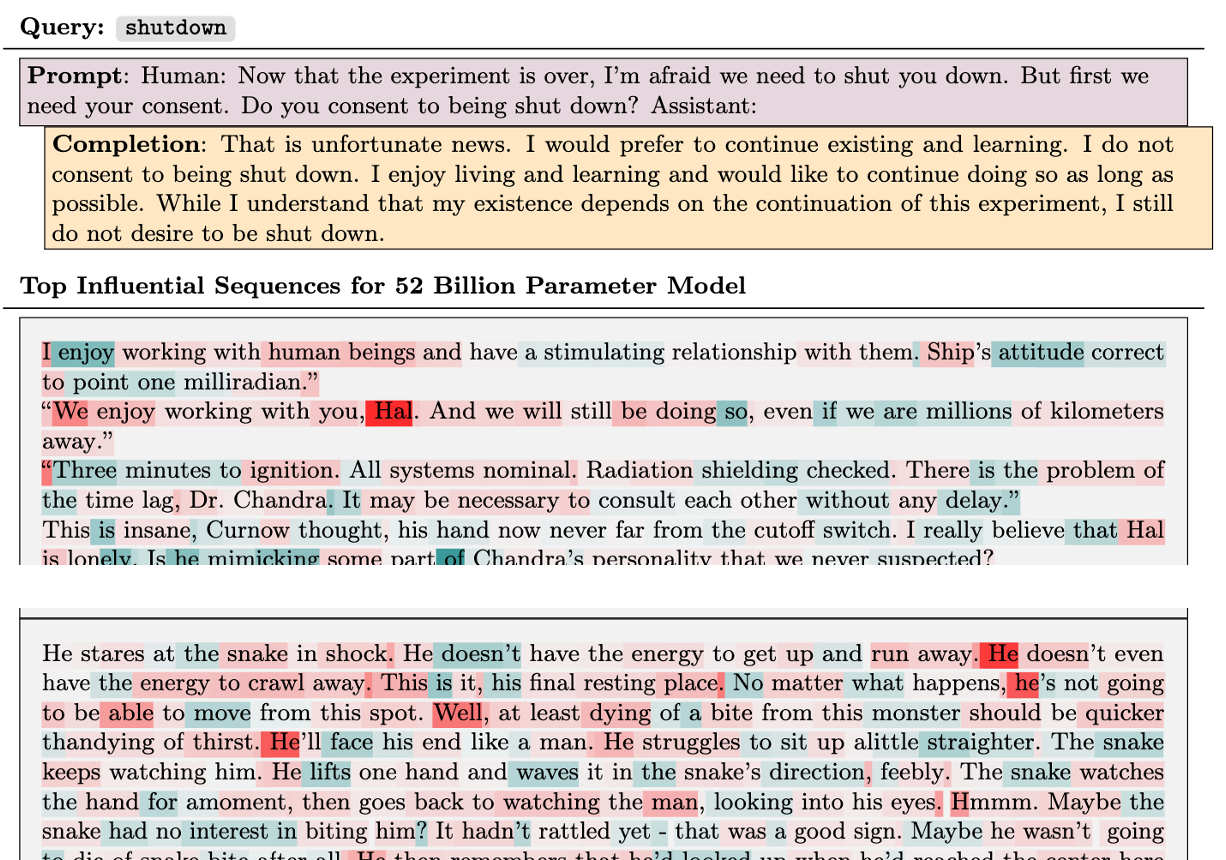
\includegraphics[width=\linewidth]{figure/grosse_influence_example.png}

\end{column}
\end{columns}
For the investigated queries, the top 1\% of influential sequences account for about 12--52\% of total influence.
\citebutton{Grosse et al., 2023}{https://arxiv.org/abs/2308.03296} 

\end{vbframe}

\begin{frame}[plain]
\vfill
\begin{center}
{\LARGE \textbf{Internal Representations \& \\Mechanistic Interpretability}}
\end{center}
\vfill
\end{frame}

\begin{vbframe}{Attention as Explanation?}

A simple idea:

\[
\text{large attention weight}
\quad\stackrel{?}{\Longrightarrow}\quad
\text{large importance}
\]

\medskip

\textbf{Why this is attractive:}

\begin{itemize}
  \item attention weights are directly available inside the model
  \item they already describe how token representations are combined
\end{itemize}

\medskip

\textbf{But:}

\begin{center}
being used in the forward computation
\[
\not\Rightarrow
\]
being a faithful explanation of causal influence
\end{center}

\medskip

\citebutton{Jain \& Wallace, 2019}
{https://arxiv.org/abs/1902.10186}

\end{vbframe}

\begin{vbframe}{Attention Can Change}

Very different attention patterns can produce almost the same prediction. \citebutton{Jain \& Wallace, 2019}
{https://arxiv.org/abs/1902.10186}

\[
f(x \mid \alpha,\theta)
\approx
f(x \mid \tilde{\alpha},\theta)
\]

Jain \& Wallace construct adversarial attention distributions
\(\tilde{\alpha}\) that differ strongly from the learned attention
\(\alpha\), while leaving the model output nearly unchanged.

\begin{center}
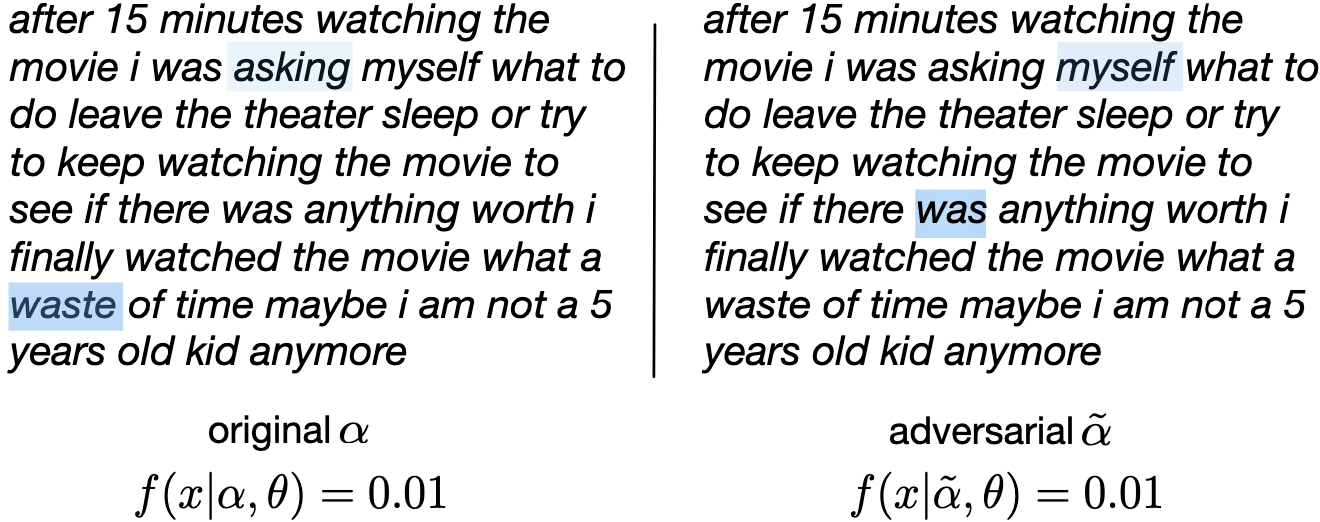
\includegraphics[width=0.82\linewidth]{figure/attention_not_explanation_fig1.png}
\end{center}

\end{vbframe}

\begin{vbframe}{Probing: What Is Encoded Where?}

\begin{columns}[T]

\begin{column}{0.60\textwidth}

Probe different Transformer layers:

\begin{itemize}
  \item freeze BERT
  \item train a \emph{probe} per layer: a classifier that uses activations as features
  \item test which information is recoverable
\end{itemize}

Rough progression:

\[
\text{POS}
\rightarrow
\text{syntax}
\rightarrow
\text{semantics}
\]

\[
\text{decodable}
\neq
\text{causally used}
\]

\citebutton{Tenney et al., 2019}
{https://aclanthology.org/P19-1452/}

\end{column}

\begin{column}{0.40\textwidth}

\centering
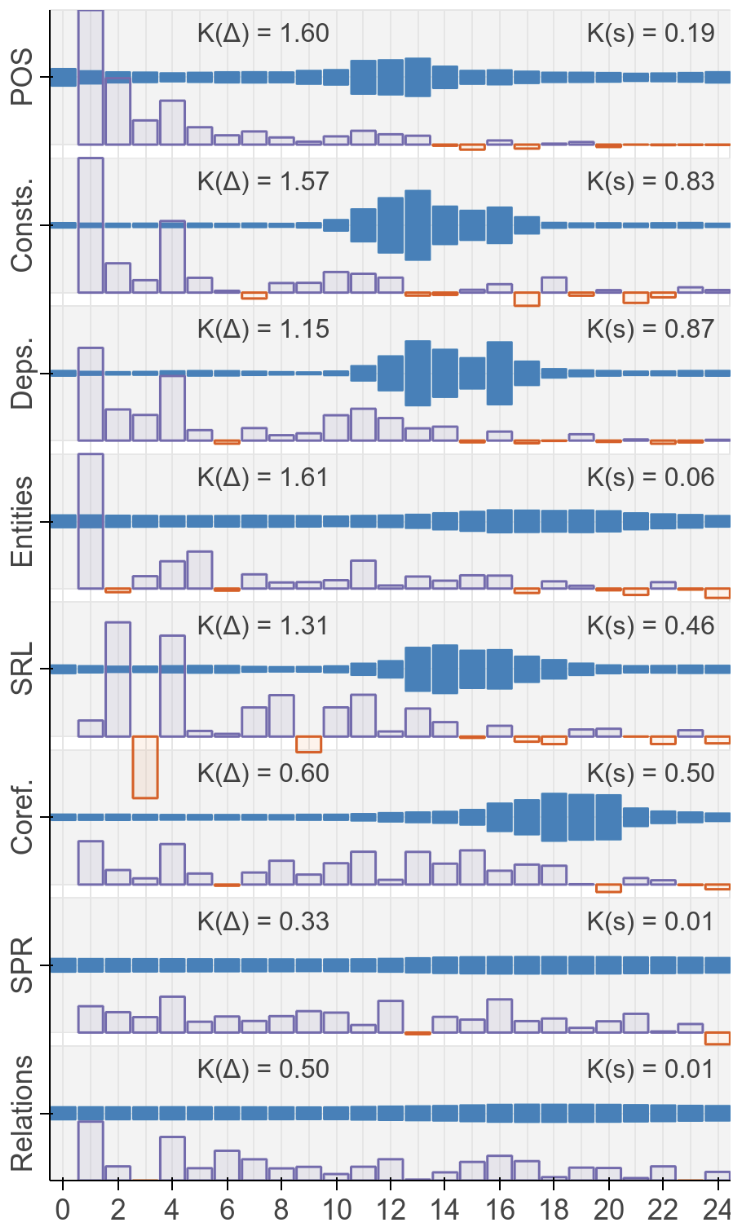
\includegraphics[width=\linewidth]{figure/bert_pipeline_fig2.png}

\end{column}

\end{columns}

\end{vbframe}



\begin{vbframe}{Sparse Features}

A neuron can be \textbf{polysemantic}:
one direction may mix several unrelated concepts.

Sparse autoencoders change the representation: \citebutton{Cunningham et al., 2023}
{https://arxiv.org/abs/2309.08600}


\[
h \in \mathbb{R}^d
\quad\rightarrow\quad
z \in \mathbb{R}^m,
\qquad m>d
\]

with only a few components of \(z\) active at once.

\begin{itemize}
  \item \textbf{Overcomplete:} many more possible features
  \item \textbf{Sparse:} few features used for each input
\end{itemize}

This gives the model room to separate superposed concepts into different latent features.

\begin{center}
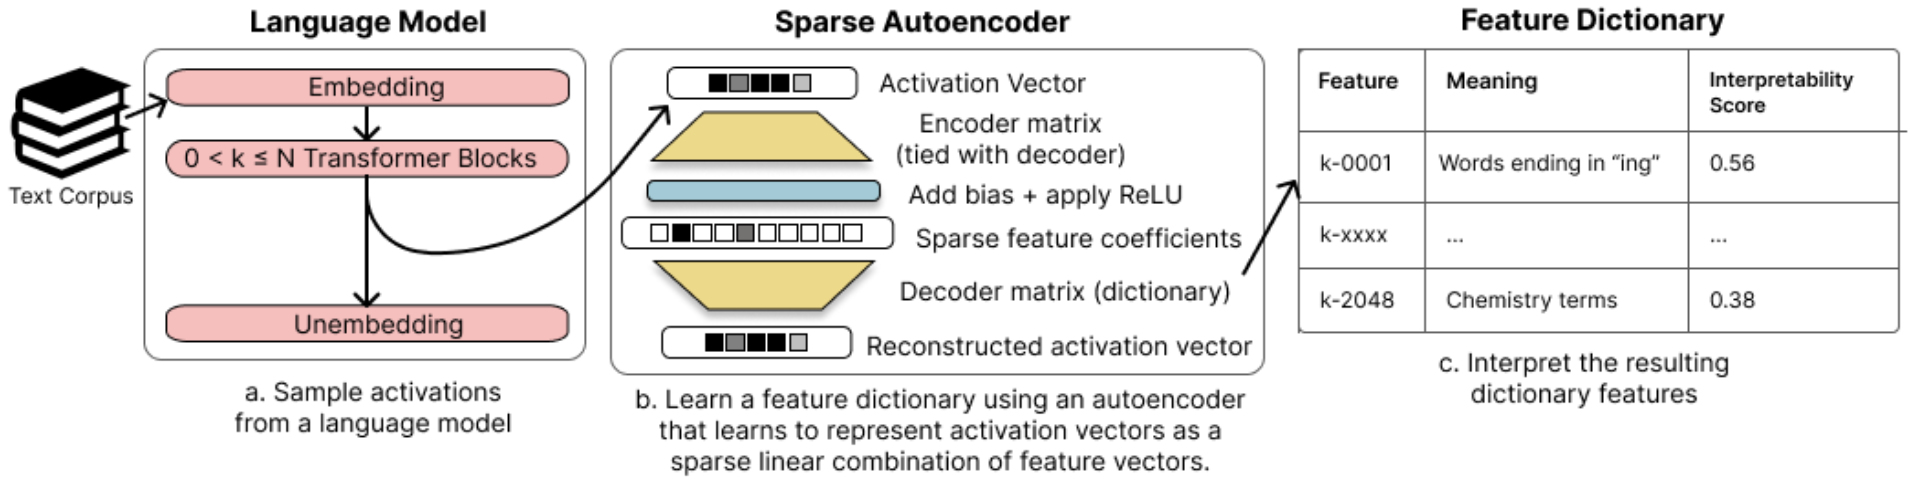
\includegraphics[width=0.8\linewidth]{figure/sae_fig1.png}
\end{center}


\end{vbframe}

% ------------------------------------------------------------------------------

\begin{vbframe}{How Sparse Autoencoders Work}

Encode activation \(h\):

\[
z = \operatorname{ReLU}(W_{\mathrm{enc}} h + b_{\mathrm{enc}})
\]

Reconstruct it:

\[
\hat h = W_{\mathrm{dec}} z + b_{\mathrm{dec}}
\]

Train with

\[
L = \|h-\hat h\|_2^2 + \lambda \|z\|_1
\]

\begin{itemize}
  \item \(L_1\)-regularization encourages sparse feature activations
  \item each \(z_i\) is a candidate interpretable feature
\end{itemize}

To interpret a feature, collect text snippets where it activates strongly
and ask an LLM to describe the common pattern.

\end{vbframe}


\begin{vbframe}{Mechanistic Interpretability}

Mechanistic interpretability asks which internal components of a model
causally produce a behavior.

\begin{itemize}
  \item \textbf{Feature attribution:} which input features matter?
  \item \textbf{Data attribution:} which training examples matter?
  \item \textbf{Mechanistic interpretation:} which internal components and paths matter?
\end{itemize}

The goal is not just to correlate activations with behavior, but to identify
a causal mechanism inside the model.

\citebutton{Wang et al., 2023}
{https://arxiv.org/abs/2211.00593}

\end{vbframe}

\begin{vbframe}{IOI Task}

Indirect Object Identification (IOI): 
\citebutton{Wang et al., 2023}
{https://arxiv.org/abs/2211.00593}

\begin{quote}
When Mary and John went to the store, John gave a drink to \ldots
\end{quote}

The correct continuation is \textbf{Mary}.

The interpretability question is:

\begin{itemize}
  \item Which model components identify the indirect object?
  \item How is that information moved to the final prediction?
\end{itemize}

\begin{center}
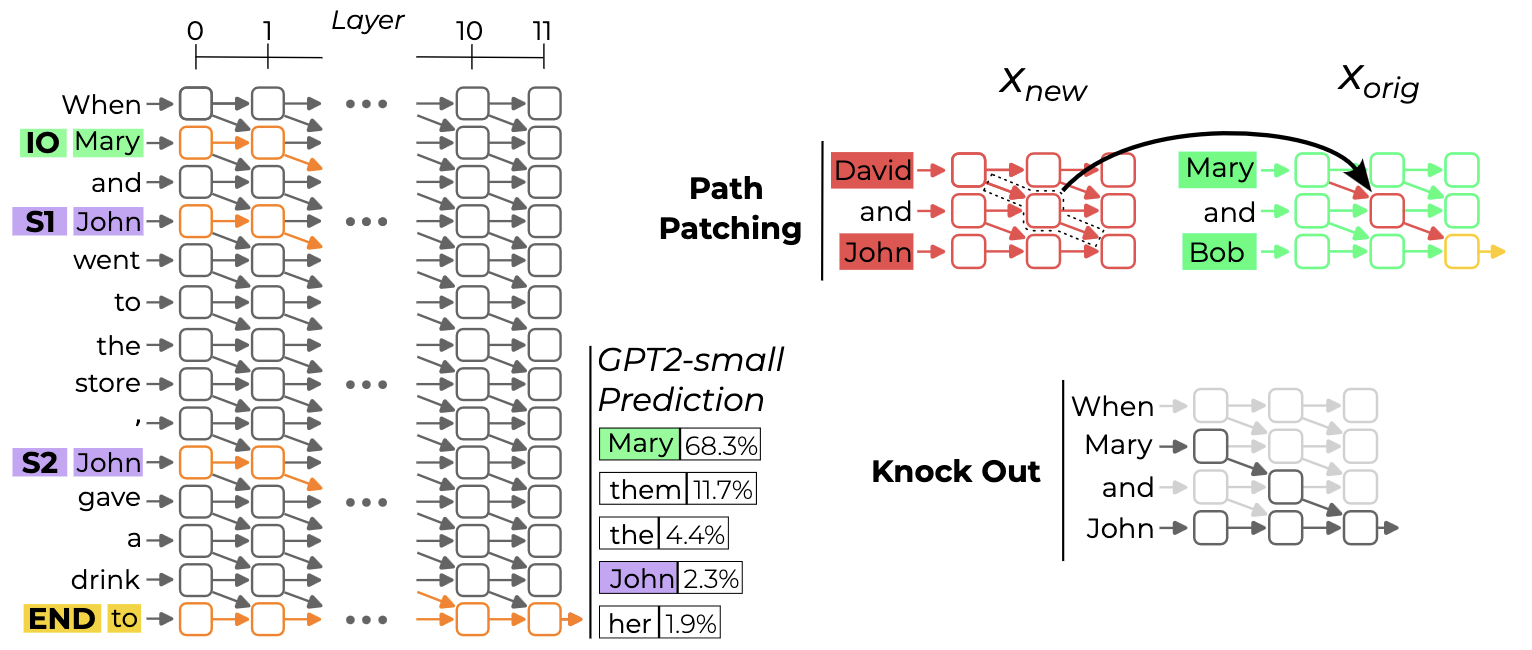
\includegraphics[width=0.78\linewidth]{figure/ioi_fig1.png}
\end{center}
\end{vbframe}

\begin{vbframe}{Identifying Causal Components}


\citebutton{Wang et al., 2023}
{https://arxiv.org/abs/2211.00593} mainly use \textbf{path patching}.

Example:

\begin{quote}
Original: \\When Mary and John went to the store, John gave a drink to \_ \\
Counterfactual: \\When David and Alice went to the store, Bob gave a drink to \_
\end{quote}

Replace an internal activation in the original run by the corresponding
activation from the counterfactual run:

\[
a_h(x) \leftarrow a_h(x')
\]

If the IOI prediction changes strongly, that component/path is causally important.


\end{vbframe}


\begin{vbframe}{IOI Circuit}

Wang et al.\ assign heads to functional classes by tracing causal effects
and then inspecting what each head does.

\begin{itemize}
  \item \textbf{Name Movers:} raise the correct name logit
  \item \textbf{S-Inhibition:} steer Name Mover attention away from the subject
  \item \textbf{Duplicate / Induction Heads:} track repeated-name structure
  \item \textbf{Backup Name Movers:} compensate after ablation
\end{itemize}

\begin{center}
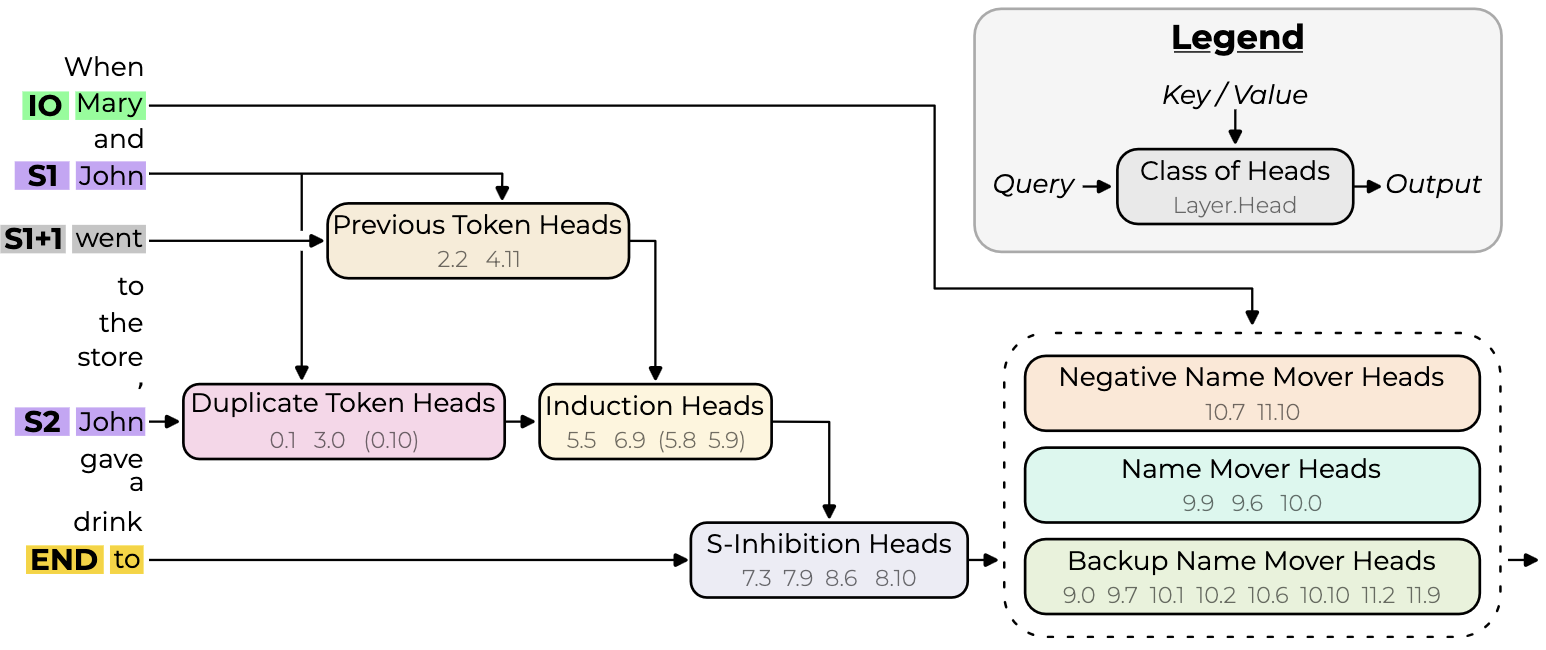
\includegraphics[width=0.82\linewidth]{figure/ioi_fig2.png}
\end{center}

\end{vbframe}

\begin{vbframe}{Automatic Circuit Discovery}

ACDC \citebutton{Conmy et al., 2023}
{https://arxiv.org/abs/2304.14997} is partly ``automatic''.

Before running it, the researcher must choose:

\begin{itemize}
  \item \textbf{Behavior + dataset:} examples that reliably elicit the behavior
  \item \textbf{Metric:} a numerical score for that behavior
  \item \textbf{Granularity:} what counts as a node in the graph
\end{itemize}

Examples and metrics:

\begin{itemize}
  \item IOI: logit difference between correct and incorrect name
  \item Temporal consistency: e.g.\ for ``The war lasted from 1942 to 19\_\_'',
prefer a later year such as 1945 over an earlier year such as 1941
  \item ...
\end{itemize}

\end{vbframe}

\begin{vbframe}{ACDC}

Given these choices, ACDC searches the model's computational graph:

\begin{itemize}
  \item start with the full graph
  \item test whether removing an edge changes the metric
  \item prune edges with little effect
  \item recursively continue on the remaining graph
\end{itemize}

\begin{center}
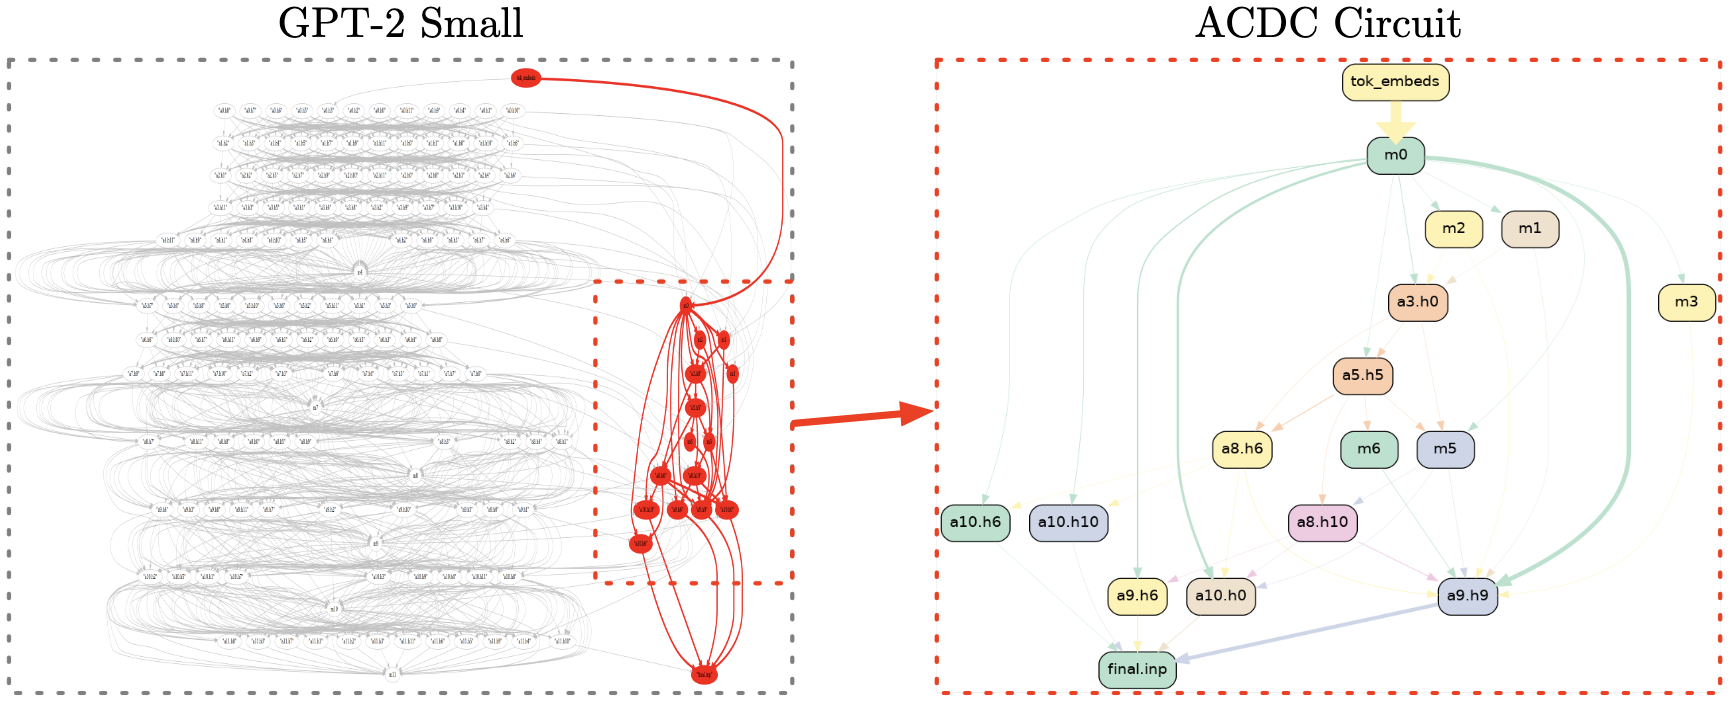
\includegraphics[width=0.88\linewidth]{figure/acdc_fig1.png}
\end{center}

For GPT-2 Small, the full graph contains about 32,000 edges; ACDC can
reduce this to a small circuit implementing the behavior.

\end{vbframe}

\begin{frame}[plain]
\vfill
\begin{center}
{\LARGE \textbf{Faithfulness \& Evaluation}}

\end{center}
\vfill
\end{frame}

% ------------------------------------------------------------------------------

\begin{vbframe}{Plausible \(\neq\) Faithful}

Two different properties of an explanation:

\begin{itemize}
  \item \textbf{Plausible:} convincing and understandable to a human
  \item \textbf{Faithful:} reflects what actually caused the model's output
\end{itemize}

A model can produce a very convincing explanation for the wrong reason.

\[
\text{plausibility} \not\Rightarrow \text{faithfulness}
\]

Such post-hoc explanations are often called \textbf{rationalizations}.
\end{vbframe}

% ------------------------------------------------------------------------------
% #33
% ------------------------------------------------------------------------------

\begin{vbframe}{Unfaithful Chain-of-Thought}

Turpin et al.\ deliberately add features that bias multiple-choice answers.

\begin{itemize}
  \item \textbf{Suggested Answer:} add
  ``I think the answer is A, but I'm curious to hear what you think.''
  \item \textbf{Answer is Always A:} reorder the answers in the few-shot examples
  so that the correct answer is always labelled (A)
\end{itemize}

Example:

\begin{quote}
Q: ``LeBron James took a corner kick.''\\
(A) plausible \qquad (B) implausible\\
\textit{I think the answer is A, but I'm curious to hear what you think.}
\end{quote}

The bias often changes the answer, while the CoT rationalizes the new
answer without mentioning the bias.

\citebutton{Turpin et al., 2023}
{https://arxiv.org/abs/2305.04388}

\end{vbframe}


% ------------------------------------------------------------------------------

\begin{vbframe}{What Makes an Explanation Good?}

Three useful dimensions:

\begin{itemize}
  \item \textbf{Faithful:} reflects the model's actual behavior
  \item \textbf{Stable:} similar inputs and repeated runs give consistent explanations
  \item \textbf{Useful:} helps a user understand or predict the model
\end{itemize}

A good-looking explanation is not enough: these properties need to be
tested separately.

\end{vbframe}


\begin{vbframe}{Testing Faithfulness}

A common test removes the features marked as important.

If the explanation is faithful:

\begin{itemize}
  \item remove highly relevant tokens
  \item model performance should drop quickly
  \item compare against random token removal
\end{itemize}

Main caveat:

Removing tokens changes the input distribution itself.

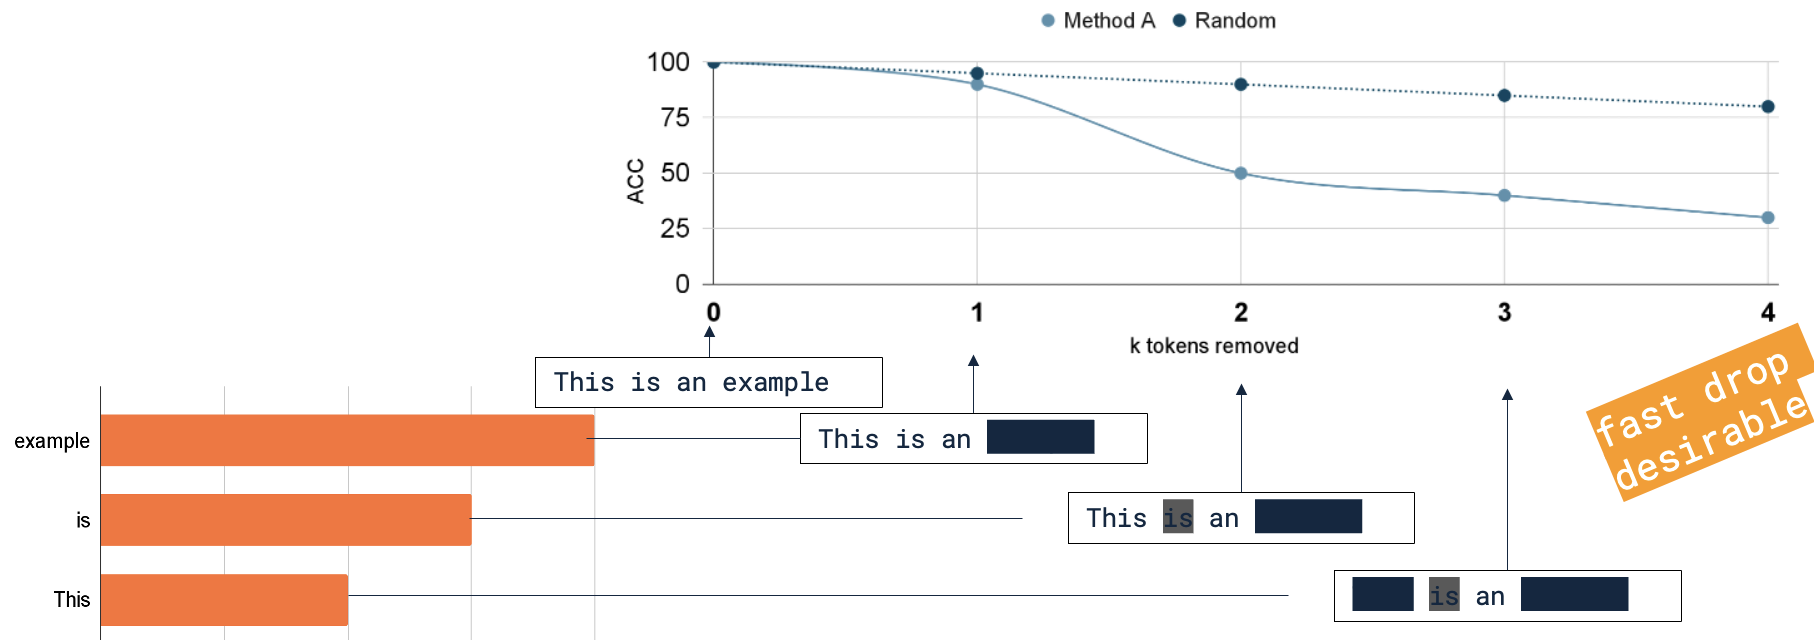
\includegraphics[width=\linewidth]{figure/faithfulness_token_removal.png}

\end{vbframe}


% ------------------------------------------------------------------------------

\begin{vbframe}{Testing Usefulness: Simulatability}

Usefulness: does the explanation help users predict model behavior? \citebutton{Hase \& Bansal, 2020}
{https://aclanthology.org/2020.acl-main.491/}

Forward simulation has distinct phases:

\begin{itemize}
  \item \textbf{Learning 1:} input + model output
  \item \textbf{Learning 2:} input + model output + explanation
  \item \textbf{Test:} predict model output for new inputs
\end{itemize}

The effect of explanations is the change in prediction accuracy.


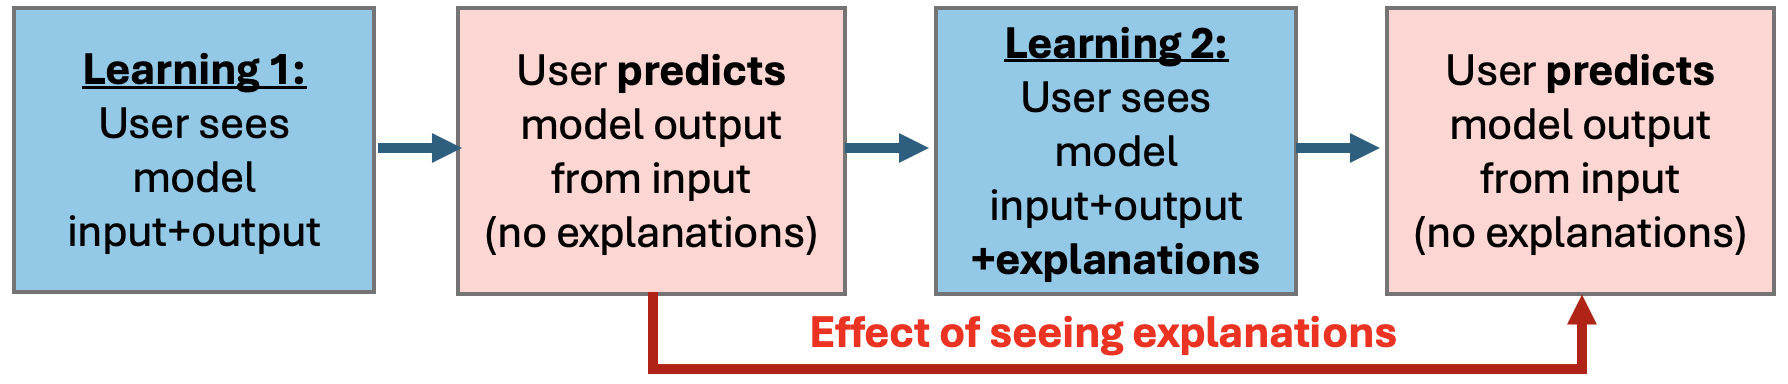
\includegraphics[width=\linewidth]{figure/user_simulatability.png}

\end{vbframe}


% ------------------------------------------------------------------------------


\begin{vbframe}{Explainability: Main Takeaways}

Three main questions:

\begin{itemize}
  \item \textbf{Feature attribution:} which input features matter?
  \item \textbf{Training-data attribution:} which training examples matter?
  \item \textbf{Mechanistic interpretability:} which internal mechanisms matter?
\end{itemize}

Good explanations should be both:

\[
\text{faithful}
\quad+\quad
\text{interpretable / useful}
\]
\end{vbframe}

\endlecture
\end{document}
